%!TEX TS-program = xelatex
%\documentclass[newPxFont]{beamer}
%\documentclass[newPxFont,handout]{beamer} % Раздаточный материал (на слайдах всё сразу)
\documentclass[aspectratio=169]{beamer} % Соотношение сторон


\usetheme{LTX}

%-=-=-=-=-=-=-=-=-=-=-=-=-=-=-=-=-=-=-=-=-=-=-=-=
%        LOADING PACKAGES
%-=-=-=-=-=-=-=-=-=-=-=-=-=-=-=-=-=-=-=-=-=-=-=-=
\usepackage{amsmath,amsfonts,amssymb,amsthm,mathtools}  % Тут мы подключаем пакеты для математики!
\usepackage{wasysym}
%%%%%%%%%%%%%%%%%%%%%%%% Шрифты %%%%%%%%%%%%%%%%%%%%%%%%%%%%%%%%%

\usepackage{fontspec}         % пакет для подгрузки шрифтов
\setmainfont{Helvetica}  % задаёт основной шрифт документа

% why do we need \newfontfamily:
% http://tex.stackexchange.com/questions/91507/
\newfontfamily{\cyrillicfonttt}{Helvetica}
\newfontfamily{\cyrillicfont}{Helvetica}
\newfontfamily{\cyrillicfontsf}{Helvetica}
% Иногда тех не видит структуры шрифтов. Эти трое бравых парней спасают ситуацию и доопределяют те куски, которые Тех не увидел.

% \usepackage{unicode-math}     % пакет для установки математического шрифта
% \setmathfont{Asana Math}      % шрифт для математики

\usepackage{polyglossia}      % Пакет, который позволяет подгружать русские буквы
\setdefaultlanguage{russian}  % Основной язык документа
\setotherlanguage{english}    % Второстепенный язык документа

%%% Работа с картинками
\usepackage{graphicx}  % Для вставки рисунков
\graphicspath{{images/}{images2/}}  % папки с картинками
\setlength\fboxsep{3pt} % Отступ рамки \fbox{} от рисунка
\setlength\fboxrule{1pt} % Толщина линий рамки \fbox{}
\usepackage{wrapfig} % Обтекание рисунков текстом

%%% Работа с таблицами
\usepackage{array,tabularx,tabulary,booktabs} % Дополнительная работа с таблицами
\usepackage{longtable}  % Длинные таблицы
\usepackage{multirow} % Слияние строк в таблице

%%% Программирование
\usepackage{etoolbox} % логические операторы

%%% Другие пакеты
\usepackage{multicol} % Несколько колонок

%%% Картинки
\usepackage{tikz} % Работа с графикой
\usepackage{pgfplots}
\usepackage{pgfplotstable}


\usepackage{xcolor}
\usepackage{hyperref}
\hypersetup{				
    unicode=true,           % позволяет использовать юникодные символы
    colorlinks=true,       	% true - цветные ссылки, false - ссылки в рамках
    urlcolor=blue,          % цвет ссылки на url
    linkcolor=red,          % внутренние ссылки
	hyperindex=true,        % сделать ли ссылку кликабельной?
	breaklinks=true         % если ссылка не умещается в одну строку, разбивать    
	                        % ли ее на две части?
}
\usepackage{verbatim}
\usepackage{fancyvrb}
\usepackage{mdframed}

 
\usepackage{chronology}

\renewcommand{\event}[3][e]{%
  \pgfmathsetlength\xstop{(#2-\theyearstart)*\unit}%
  \ifx #1e%
    \draw[fill=black,draw=none,opacity=0.5]%
      (\xstop, 0) circle (.2\unit)%
      node[opacity=1,rotate=45,right=.2\unit] {#3};%
  \else%
    \pgfmathsetlength\xstart{(#1-\theyearstart)*\unit}%
    \draw[fill=black,draw=none,opacity=0.5,rounded corners=.1\unit]%
      (\xstart,-.1\unit) rectangle%
      node[opacity=1,rotate=45,right=.2\unit] {#3} (\xstop,.1\unit);%
  \fi}%


\title{Уютный факультатив по \LaTeX}
\subtitle{Картинки, таблицы, графика}
\date{\today}

\begin{document}


\maketitle
 
\section{Картинки} 

\begin{frame}{Векторные и растровые картинки} 
\begin{columns}
\begin{column}{.55\linewidth}
\begin{itemize}
\item Растровые: PNG, GIF, JPEG \ldots
\item Хранятся пиксельно, немасштабируются
\item Веторные: PDF, EPS \ldots
\item Хранятся описательно, масштабируются
\item Сложный объект требует много места векторно и мало растрово.
\end{itemize}
\end{column}
\begin{column}{.42\linewidth}

\includegraphics[width=0.99\linewidth]{rv.jpg}
\end{column}
\end{columns}
\end{frame}


\begin{frame}[fragile]{ }
\begin{block}{Единицы измерения в \LaTeX}
\centering 
	\begin{tabulary}{\textwidth}{JccL}
		\toprule
			pt & & &пункт (0.35 mm) \\
			pc & & &пика  (12 pt)   \\
			mm & & &миллиметр       \\
			cm & & &сантиметр       \\
			in & & &дюйм            \\
			em & & &ширина буквы M используемого шрифта \\
			ex & & &высота буквы x используемого шрифта \\
		\bottomrule
	\end{tabulary}
\end{block}
\end{frame}


\begin{frame}[fragile]{ }
\begin{block}{И ещё немного длин в \LaTeX}
\centering 
	\begin{tabulary}{\textwidth}{JccL}
		\toprule
			\verb|\pagewidth|  & & &ширина страницы \\
			\verb|\pageheight| & & &высота страницы \\
			\verb|\textwidth|  & & &ширина текста   \\
			\verb|\textheight| & & &высота текста   \\
			\verb|\linewidth|  & & & длина текста в текущем окружении \\
		\bottomrule
	\end{tabulary}
\end{block}
\end{frame} 

\begin{frame}[fragile]{ }
\begin{block}{Рисунок! Знай своё место!}
\centering 
	\begin{tabulary}{\textwidth}{JL}
		\toprule
			с & поставить рисунок где удобно \TeX у и поместить его в центре (center) \\
			t & поставить рисунок где удобно \TeX у и прижать его к верху (top) \\
			b & поставить рисунок где удобно \TeX у и прижать его к низу   (bottom) \\
			p & поставить рисунок на отдельной странице, целиком состоящей из "плавающих" рисунков и таблиц \\
			h & поставить рисунок там, где он идет по тексту с нарушением всех правил верстки (here)  \\
		   h! & поставить ну прям с высокой вероятностью там где надо нам \\
			H & в 100 случаях из 100 рисунок будет там где нам надо (нужно подгрузить пакет float) \\
		\bottomrule
	\end{tabulary}
\end{block}
\end{frame} 


\section{Таблицы} 

% показать как в texmaker вставлять шаблон с таблицей! Quick Tabular

\begin{frame}
\begin{block}{Типы колонок в таблицах}
\centering 
	\begin{tabulary}{\textwidth}{JL}
		\toprule
			c & колонка выровнена по центру \\
			l & колонка выровнена по левому краю\\
			r & колонка выровнена по правому краю\\
	   p\{ \} & колонка создаётся как абзац, в скобках ширина колонки \\
		   X  & подбирает столбцы равной ширины (tabularx) \\
		   C  & одинаково строк во всех столбцах, выравнивание по центру  \\	  
		   J  & одинаково строк во всех столбцах, выравнивание по ширине \\
		   R  & одинаково строк во всех столбцах, выравнивание по правому краю \\
		   L  & одинаково строк во всех столбцах, выравнивание по левому краю  \\
		\bottomrule
	\end{tabulary}
\end{block}
\vspace{0.1cm} \centering
\large Последние четыре команды лежат в пакете tabulary

\alert{Не забывайте о существовании Quick Tabular \ldots}

\end{frame}

\begin{frame}{Читаемые и нечитаемые таблицы} 
\begin{columns}
\begin{column}{.49\linewidth}
\tiny
\begin{tabular}{|r|r|r|r|r|}
\hline
& Estimate & Std. Error & t value & $Pr( > | t |)$ \\
\hline
Intercept & -1.6598 & 0.0239 & -69.51 & 0.0000 \\ \hline
cut & -0.0206 & 0.0014 & -14.53 & 0.0000 \\ \hline
color & 0.1085 & 0.0011 & 97.30 & 0.0000 \\ \hline
clarity & -0.1784 & 0.0021 & -86.67 & 0.0000 \\ \hline
depth & 0.0121 & 0.0003 & 43.28 & 0.0000 \\ \hline
table & 0.0022 & 0.0002 & 12.07 & 0.0000 \\ \hline
price & 0.0000 & 0.0000 & 231.49 & 0.0000 \\ \hline
x & 0.2425 & 0.0018 & 134.73 & 0.0000 \\ \hline
y & 0.0060 & 0.0012 & 4.92 & 0.0000 \\ \hline
z & 0.0046 & 0.0021 & 2.18 & 0.0290 \\ 
\hline
\end{tabular}
\end{column}
\begin{column}{.49\linewidth}
\tiny
\begin{tabular}{rrrrr}
\toprule
& Estimate & Std. Error & t value & $Pr( > | t |)$ \\
\midrule
Intercept & -1.6598 & 0.0239 & -69.51 & 0.0000 \\ 
cut & -0.0206 & 0.0014 & -14.53 & 0.0000 \\ 
color & 0.1085 & 0.0011 & 97.30 & 0.0000 \\ 
clarity & -0.1784 & 0.0021 & -86.67 & 0.0000 \\ 
depth & 0.0121 & 0.0003 & 43.28 & 0.0000 \\ 
table & 0.0022 & 0.0002 & 12.07 & 0.0000 \\ 
price & 0.0000 & 0.0000 & 231.49 & 0.0000 \\ 
x & 0.2425 & 0.0018 & 134.73 & 0.0000 \\
y & 0.0060 & 0.0012 & 4.92 & 0.0000 \\
z & 0.0046 & 0.0021 & 2.18 & 0.0290 \\ 
\bottomrule
\end{tabular}
\end{column}
\end{columns}

\vspace{1cm}
\centering
\Large
\alert{Какая из таблиц лучше? Выбор очевиден?} 
\end{frame}


\begin{frame}{Ещё пример} 
\centering
\tiny
\begin{tabular}{|c|c|c|c|c|c|c|c|} 
\hline
$m$ & $\Re\{\underline{\mathfrak{X}}(m)\}$ &$-\Im\{\underline{\mathfrak{X}}(m)\}$ & $\mathfrak{X}(m)$ & $\frac{\mathfrak{X}(m)}{23}$ & $A_m$ & $\varphi(m)\ /\ ^{\circ}$ & $\varphi_m\ /\ ^{\circ}$ \\ \hline
1  & 16.128 & +8.872 & 16.128 & 1.402 & 1.373 & -146.6 & -137.6 \\  \hline
2  & 3.442  & -2.509 & 3.442  & 0.299 & 0.343 & 133.2  & 152.4  \\  \hline
3  & 1.826  & -0.363 & 1.826  & 0.159 & 0.119 & 168.5  & -161.1 \\  \hline
4  & 0.993  & -0.429 & 0.993  & 0.086 & 0.08  & 25.6   & 90     \\  \hline
5  & 1.29   & +0.099 & 1.29   & 0.112 & 0.097 & -175.6 & -114.7 \\  \hline
6  & 0.483  & -0.183 & 0.483  & 0.042 & 0.063 & 22.3   & 122.5  \\  \hline
7  & 0.766  & -0.475 & 0.766  & 0.067 & 0.039 & 141.6  & -122   \\  \hline
\end{tabular}

\Large{\alert{И выбор снова очевиден!}}

\tiny
\begin{tabular}{cccccccc} \toprule
    {$m$} & {$\Re\{\underline{\mathfrak{X}}(m)\}$} & {$-\Im\{\underline{\mathfrak{X}}(m)\}$} & {$\mathfrak{X}(m)$} & {$\frac{\mathfrak{X}(m)}{23}$} & {$A_m$} & {$\varphi(m)\ /\ ^{\circ}$} & {$\varphi_m\ /\ ^{\circ}$} \\ \midrule
1  & 16.128 & +8.872 & 16.128 & 1.402 & 1.373 & -146.6 & -137.6 \\
 2  & 3.442  & -2.509 & 3.442  & 0.299 & 0.343 & 133.2  & 152.4  \\
 3  & 1.826  & -0.363 & 1.826  & 0.159 & 0.119 & 168.5  & -161.1 \\
4  & 0.993  & -0.429 & 0.993  & 0.086 & 0.08  & 25.6   & 90     \\
5  & 1.29   & +0.099 & 1.29   & 0.112 & 0.097 & -175.6 & -114.7 \\
6  & 0.483  & -0.183 & 0.483  & 0.042 & 0.063 & 22.3   & 122.5  \\
7  & 0.766  & -0.475 & 0.766  & 0.067 & 0.039 & 141.6  & -122   \\ \bottomrule
\end{tabular}
\end{frame}


\begin{frame}{Правила этикета для истиных Леди и Джентельменов} 
\begin{block}{Заповеди из документации к booktabs}
\begin{enumerate}
\item Будьте проще! Глазам должно быть комфортно.
\item Не используйте вертикальные линни.
\item Не используйте двойные линии. Как правило достаточно трёх горизонтальных линий.
\item Оставляйте место между строками
\item Единицы измерения - в шапку таблицы
\item Повторяющееся значение повторяйте, а не говорите "то же"
\item Если сомневаетесь, выравнивайте по левому краю!
\end{enumerate}
\end{block}
\end{frame}


\begin{frame}[plain]{Excel2LaTeX} 
\begin{center} 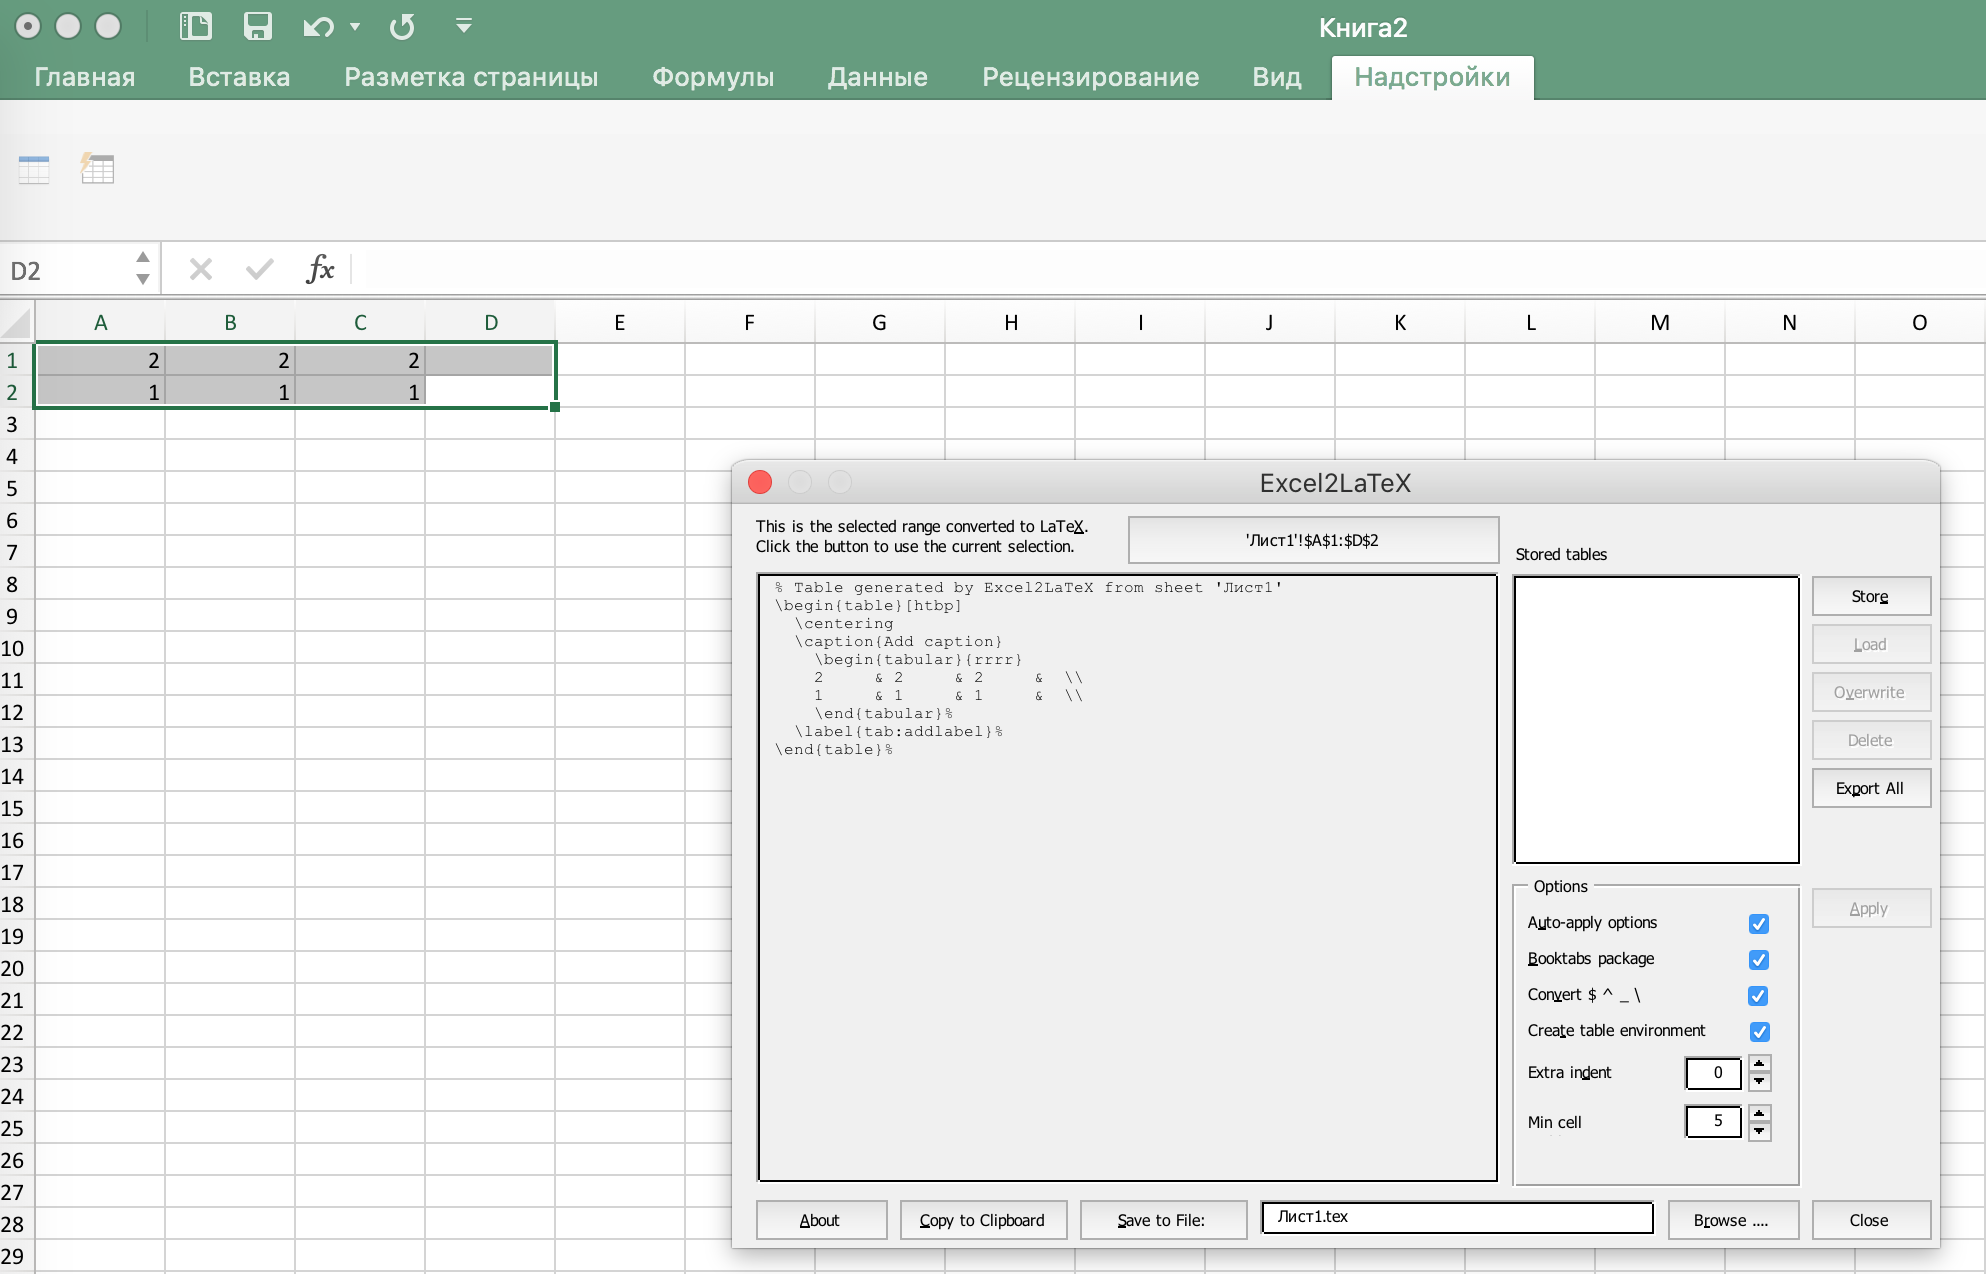
\includegraphics[width=0.45\linewidth]{excel2latex.png}	
\end{center}

\begin{block}{Ссылка на макрос:}
	\vspace{3mm}
	\centerline {\url{https://ctan.org/tex-archive/support/excel2latex}}
	\vspace{3mm}
\end{block}
\end{frame}


\section{TikZ и Geogebra} 


\begingroup
\setbeamercolor{background canvas}{bg = LTXDarkGrey}
\begin{frame}[plain]
\centering 
\includegraphics[width=0.55\linewidth]{wearlatex.png}
\end{frame}
\endgroup 
\end{document}
